\input{preamble-standalone.ltx}
\begin{document}

% Ex. No. 13 (Section  6.1 : \tkzcname{tkzDrawX}} \hypertarget{dx}{)

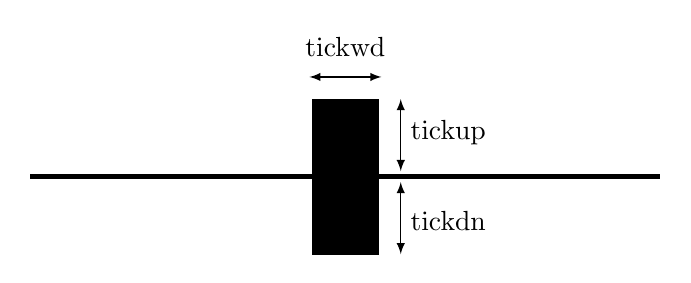
\begin{tikzpicture}[>=latex,scale=2]
  \draw[line width=2 pt](0,0)--(4,0);
  \draw[fill] (2cm-6pt,-14pt) rectangle (2cm+6pt,+14pt);
  \draw[<->](2cm-6.5pt,18pt) -- (2cm+6.5pt,+18pt);
  \node[above] at (2cm,20pt) {tickwd};
  \draw[<->](2cm+10pt,1pt) -- (2cm+10pt,+14pt);
  \node[right] at (2cm+10pt,8pt) {tickup};
  \draw[<->](2cm+10pt,-1pt) -- (2cm+10pt,-14pt);
  \node[right] at (2cm+10pt,-8pt) {tickdn};
\end{tikzpicture}

\end{document}